\documentclass[aspectratio=169, 10pt]{beamer}
\usetheme[progressbar=frametitle]{metropolis}

% Add some packages
\usepackage{appendixnumberbeamer}
\usepackage{xcolor}
\usepackage{booktabs}
\usepackage[scale=2]{ccicons}
\usepackage{tikz}
\usepackage{pgfplots}
\usepgfplotslibrary{dateplot}
\usepackage{hyperref}
\usepackage{xspace}
\usepackage[absolute,overlay]{textpos}
\usepackage{pgffor}
\usepackage{xstring}

% Use Helvetica font
\usepackage[scaled]{helvet}
\renewcommand{\familydefault}{\sfdefault}


\pgfplotsset{compat=1.15}


% Define the ORNL colors, taken from https://standards.ornl.gov/logos/
% as well as https://www.olcf.ornl.gov/olcf-media/media-assets/
\definecolor{ornlgreen}{RGB}{0,121,52}
\definecolor{ornlblack}{RGB}{0,0,0}
\definecolor{ornlgrey}{RGB}{88,88,88}
\definecolor{backgroundgreen}{RGB}{68,126,89}
\definecolor{backgroundgrey}{RGB}{191,191,191}

% Set the frame title backgrounds to be text green, background white
\setbeamercolor{palette primary}{fg=backgroundgreen, bg=white}

% Set the bar underneath the title blocks to a color
\setbeamercolor{progress bar}{fg=white,bg=white}

% Set text color
\setbeamercolor{normal text}{fg = ornlblack, bg=white}

\newcommand{\themename}{\textbf{\textsc{metropolis}}\xspace}

% Global footer to put speaker's name, if desired
\setbeamertemplate{frame footer}{\hspace*{2cm}\vspace*{-0.1cm}\footnotesize}

% Global background set, to use the default frame background
\usebackgroundtemplate{
\includegraphics[width=\paperwidth]{figs/slide_frame.png}}

% Define a new command for a mathematical symbol
\newcommand{\Xresi}{X_{\text{res}}}
\newcommand{\mdies}{m_{\text{in}}^{\text{dsl}}}
\newcommand{\mammo}{m_{\text{in}}^{\text{NH3}}}
\newcommand{\mair}{m_{\text{in}}^{\text{air}}}
\newcommand{\Qlhvd}{Q_{\text{LHV}}^{\text{dsl}}}
\newcommand{\Qlhva}{Q_{\text{LHV}}^{\text{NH3}}}
\newcommand{\Qgros}{Q_{\text{gross}}}
\newcommand{\Mfuel}{M_{\text{fuel}}}
\newcommand{\Mair}{M_{\text{air}}}

\begin{document}

%
% Title slide
%
{
\usebackgroundtemplate{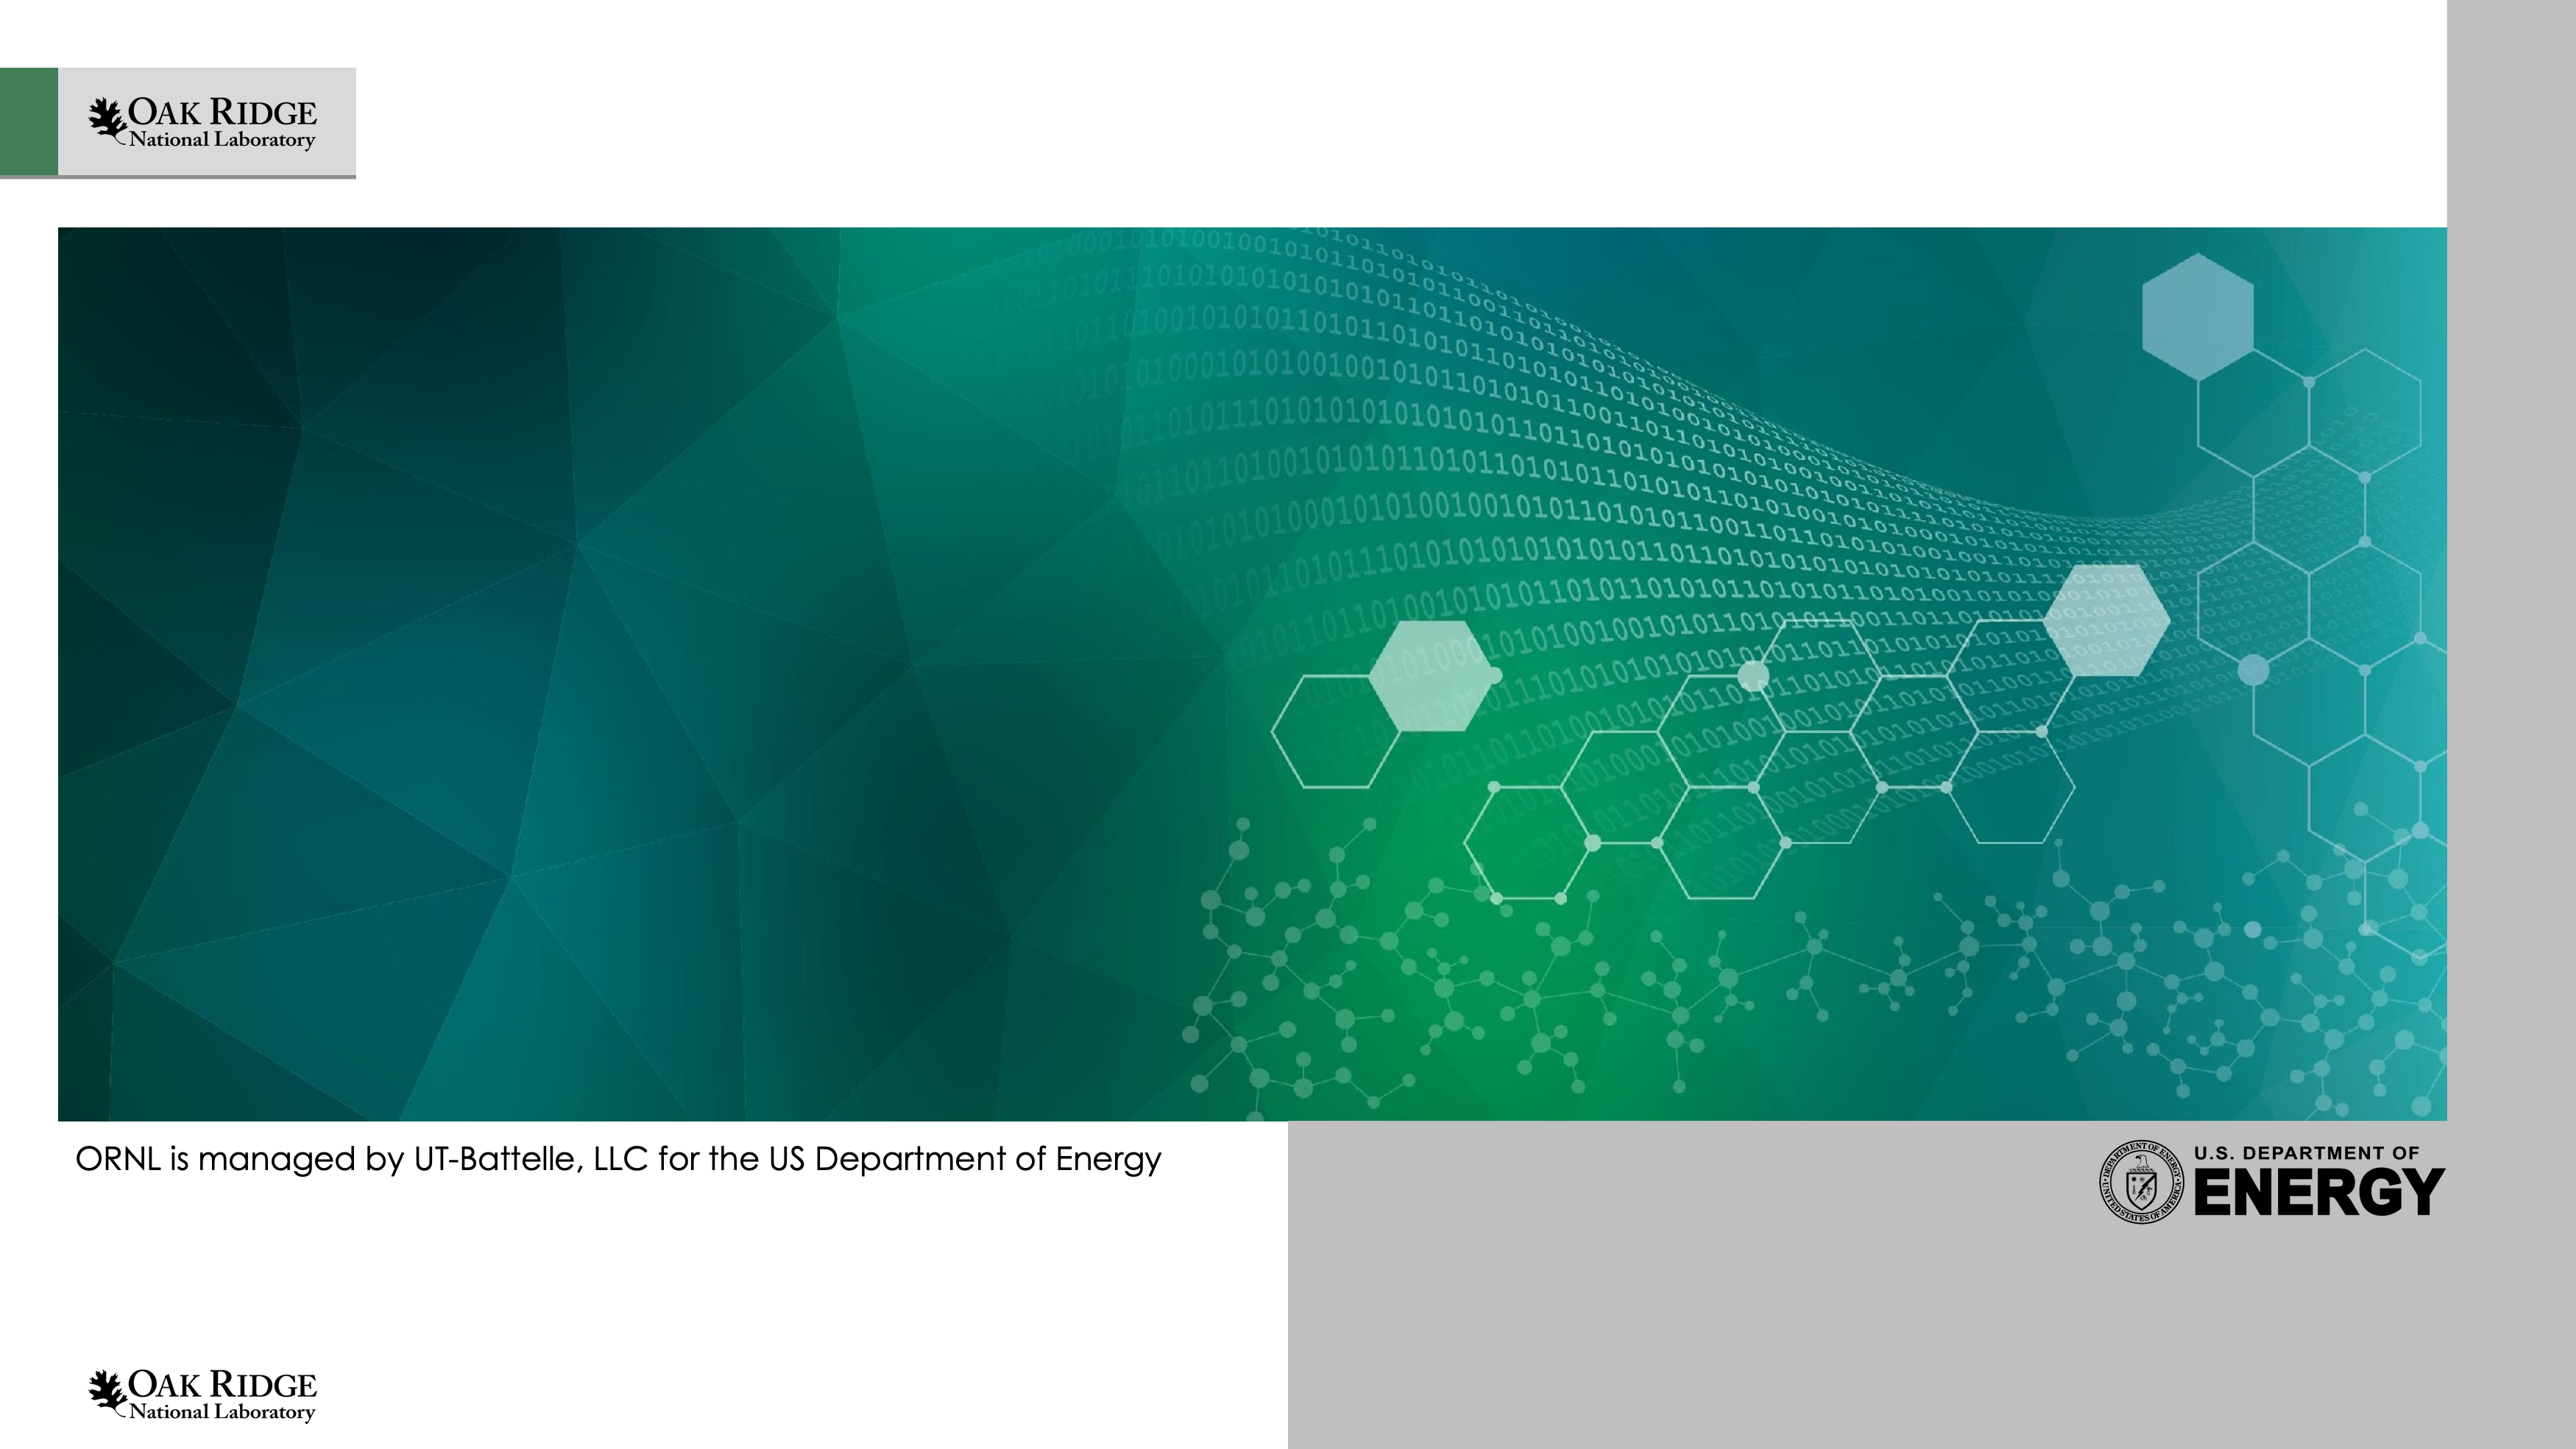
\includegraphics[width=\paperwidth]{figs/title_frame.png}}
\setbeamertemplate{footline}{}
\begin{frame}
\textcolor{white}{\Huge Ammonia-Diesel experimental data and modeling results}\\
\vspace*{0.7cm}
\textcolor{white}{\Large Bryan Maldonado}\\
\textcolor{white}{ ORNL}\\
\textcolor{white}{ \today}


\end{frame}
}

%
% Content
%
\begin{frame}
\frametitle{Ammonia-Diesel dual fuel operating conditions}
	\centering
		Baseline operating condition: 1200 rpm, 6 bar IMEPn target, 42 g/min ammonia fuel flow
		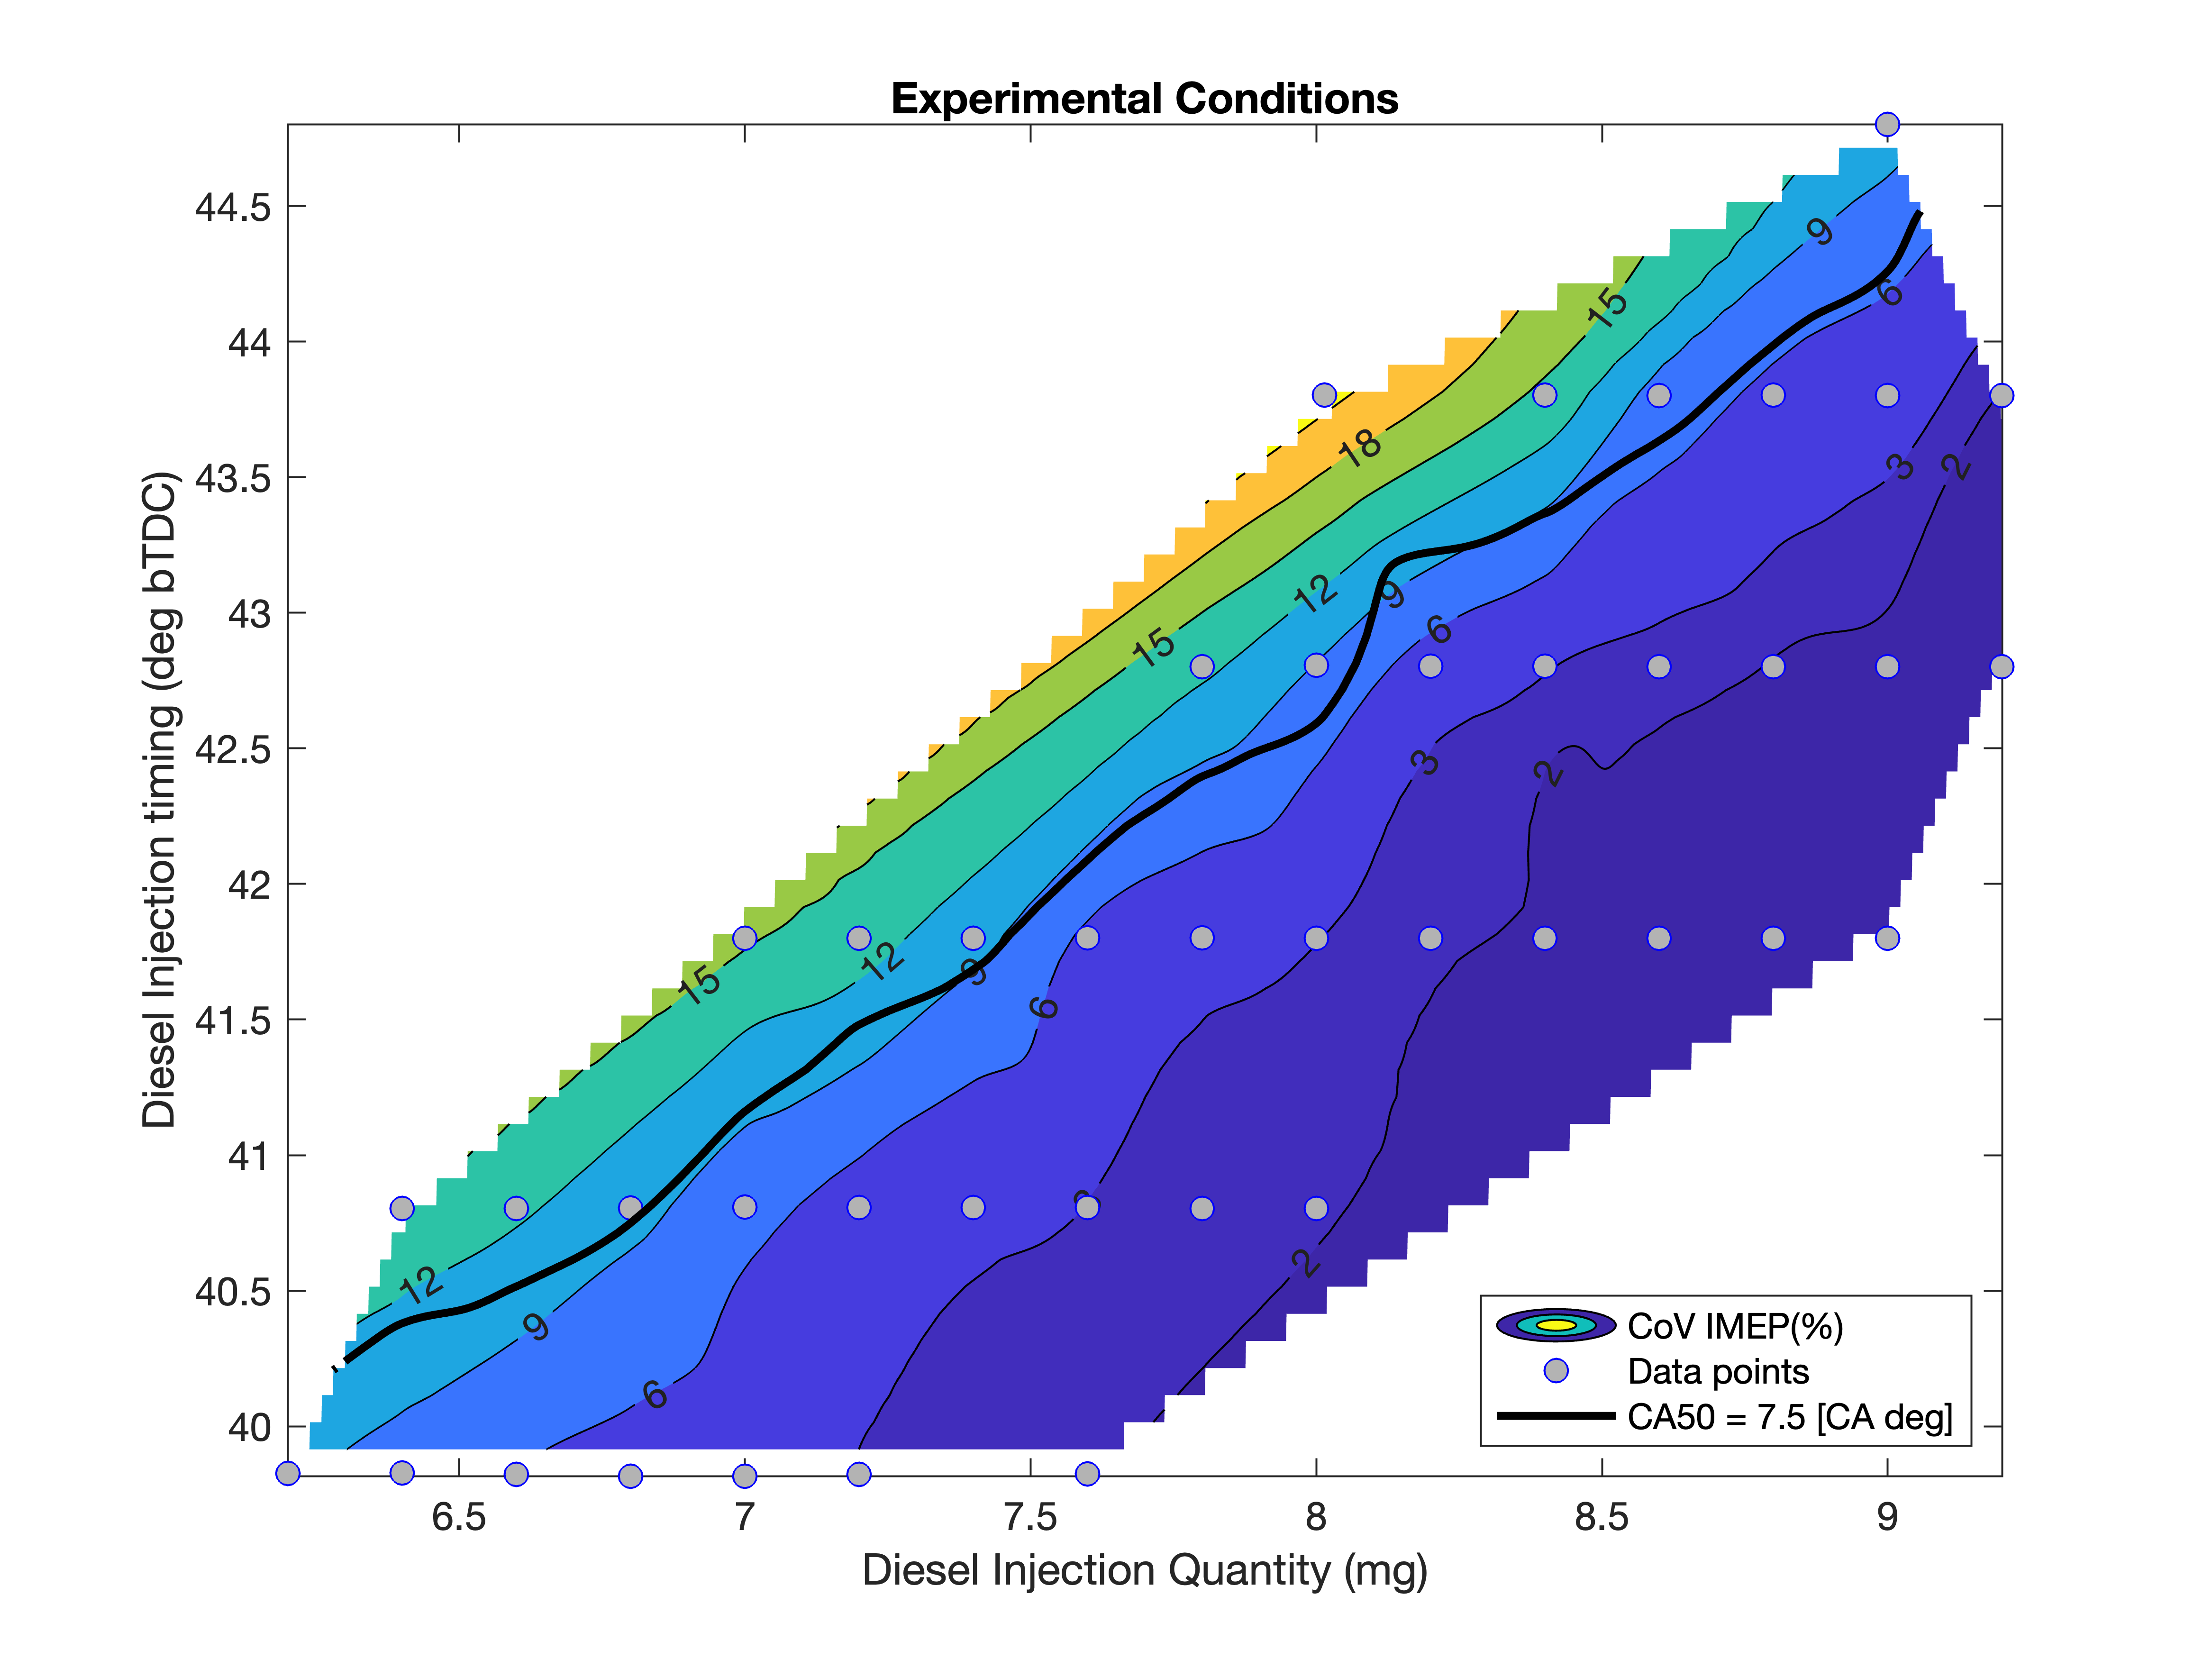
\includegraphics[height=0.85\textheight]{../Model_Plots/Overview.png}
\end{frame}

\foreach \cond in {
DI6_2_SOI40, DI6_4_SOI40, DI6_4_SOI41, DI6_6_SOI40, DI6_6_SOI41, DI6_8_SOI40, DI6_8_SOI41, DI7_0_SOI40, DI7_0_SOI41, DI7_0_SOI42, DI7_2_SOI40, DI7_2_SOI41, DI7_2_SOI42, DI7_4_SOI41, DI7_4_SOI42, DI7_6_SOI40, DI7_6_SOI41, DI7_6_SOI42, DI7_8_SOI41, DI7_8_SOI42, DI7_8_SOI43, DI8_0_SOI41, DI8_0_SOI42, DI8_0_SOI43, DI8_0_SOI44, DI8_2_SOI42, DI8_2_SOI43, DI8_4_SOI42, DI8_4_SOI43, DI8_4_SOI44, DI8_6_SOI42, DI8_6_SOI43, DI8_6_SOI44, DI8_8_SOI42, DI8_8_SOI43, DI8_8_SOI44, DI9_0_SOI42, DI9_0_SOI43, DI9_0_SOI44, DI9_0_SOI45, DI9_2_SOI43, DI9_2_SOI44}
{
% Replace underscores with spaces and store in \temp
\StrSubstitute{\cond}{_}{ }[\temp]
\StrSubstitute[1]{\temp}{ }{.}[\final]

\begin{frame}
\frametitle{\final: Estimation of combustion efficiency and in-cylinder mass}
$\eta_c = \dfrac{1 - \Xresi}{\dfrac{\mdies \Qlhvd + \mammo \Qlhva}{\Qgros} - \Xresi}$,\hspace{2em}
$\begin{array}{l}
\Mfuel = \dfrac{\mdies + \mammo - \Xresi\dfrac{\Qgros( \mdies + \mammo )}{\mdies \Qlhvd + \mammo \Qlhva}}{1 - \Xresi}\\
\Mair = \dfrac{\mair + \Xresi\dfrac{\Qgros( \mdies + \mammo )}{\mdies \Qlhvd + \mammo \Qlhva}}{1 - \Xresi}
\end{array}$
\includegraphics[width=0.49\textwidth]{../Model_Plots/\cond_eta_c.png}
\includegraphics[width=0.49\textwidth]{../Model_Plots/\cond_Mass.png}
\end{frame}

\begin{frame}
\frametitle{\final: Parametric model ($\mu_\eta, \Sigma_\eta, \mu_X, \Sigma_X$)}
\hspace{3em}$\begin{array}{l}
\begin{bmatrix} \eta_c & \Mfuel & \Mair \end{bmatrix} \sim \mathcal{N}(\mu_\eta, \Sigma_\eta) \\
\therefore \eta_c \mid \begin{bmatrix} \Mfuel & \Mair \end{bmatrix} \sim \mathcal{N}(\bar{\mu}, \bar{\Sigma})
\end{array}$,\hspace{5em}
$\begin{array}{l}
\begin{bmatrix} \Xresi & \Qgros \end{bmatrix} \sim \mathcal{N}(\mu_X, \Sigma_X) \\
\therefore \Xresi \mid \Qgros \sim \mathcal{N}(\bar{\mu}, \bar{\Sigma})
\end{array}$
\includegraphics[width=0.49\textwidth]{../Model_Plots/\cond_eta_c_model.png}
\includegraphics[width=0.49\textwidth]{../Model_Plots/\cond_X_res_model.png}
\end{frame}

\begin{frame}
\frametitle{\final: Simulator Results}
{\scriptsize
$\begin{bmatrix} \Mfuel \\ \Mair \end{bmatrix}_{k+1} = \Xresi[k]
\begin{bmatrix} 1 - \eta_c[k] & 0 \\ \eta_c[k] & 1\end{bmatrix}
\begin{bmatrix} \Mfuel \\ \Mair \end{bmatrix}_k + 
\begin{bmatrix} \mammo + \mdies[k] \\ \mair \end{bmatrix}$, 
$\Qgros[k] = \eta_c[k]\Mfuel[k]\dfrac{\mdies[k] \Qlhvd + \mammo \Qlhva}{\mdies[k] + \mammo}$}
\begin{center}
\includegraphics[height=0.85\textheight]{../Model_Plots/\cond_Simulator.png}
\end{center}
\end{frame}
}

\begin{frame}
\frametitle{Model parameter $\mu_\eta$ as function of DI strategy}
\begin{center}
\foreach \i in {1, 2, 3}{
\includegraphics[width=0.36\textwidth]{../Model_Plots/mu_eta_\i.png}
}
\end{center}
\end{frame}

\begin{frame}
\frametitle{Model parameter $\Sigma_\eta$ as function of DI strategy}
\begin{center}
\foreach \i in {1, 2, 3}{
\foreach \j in {\i, ..., 3}{
\includegraphics[width=0.32\textwidth]{../Model_Plots/Sigma_eta_\i\j.png}
}}
\end{center}
\end{frame}

\begin{frame}
\frametitle{Model parameter $\mu_X$ as function of DI strategy}
\begin{center}
\foreach \i in {1, 2}{
\includegraphics[width=0.49\textwidth]{../Model_Plots/mu_X_\i.png}
}
\end{center}
\end{frame}

\begin{frame}
\frametitle{Model parameter $\Sigma_X$ as function of DI strategy}
\begin{center}
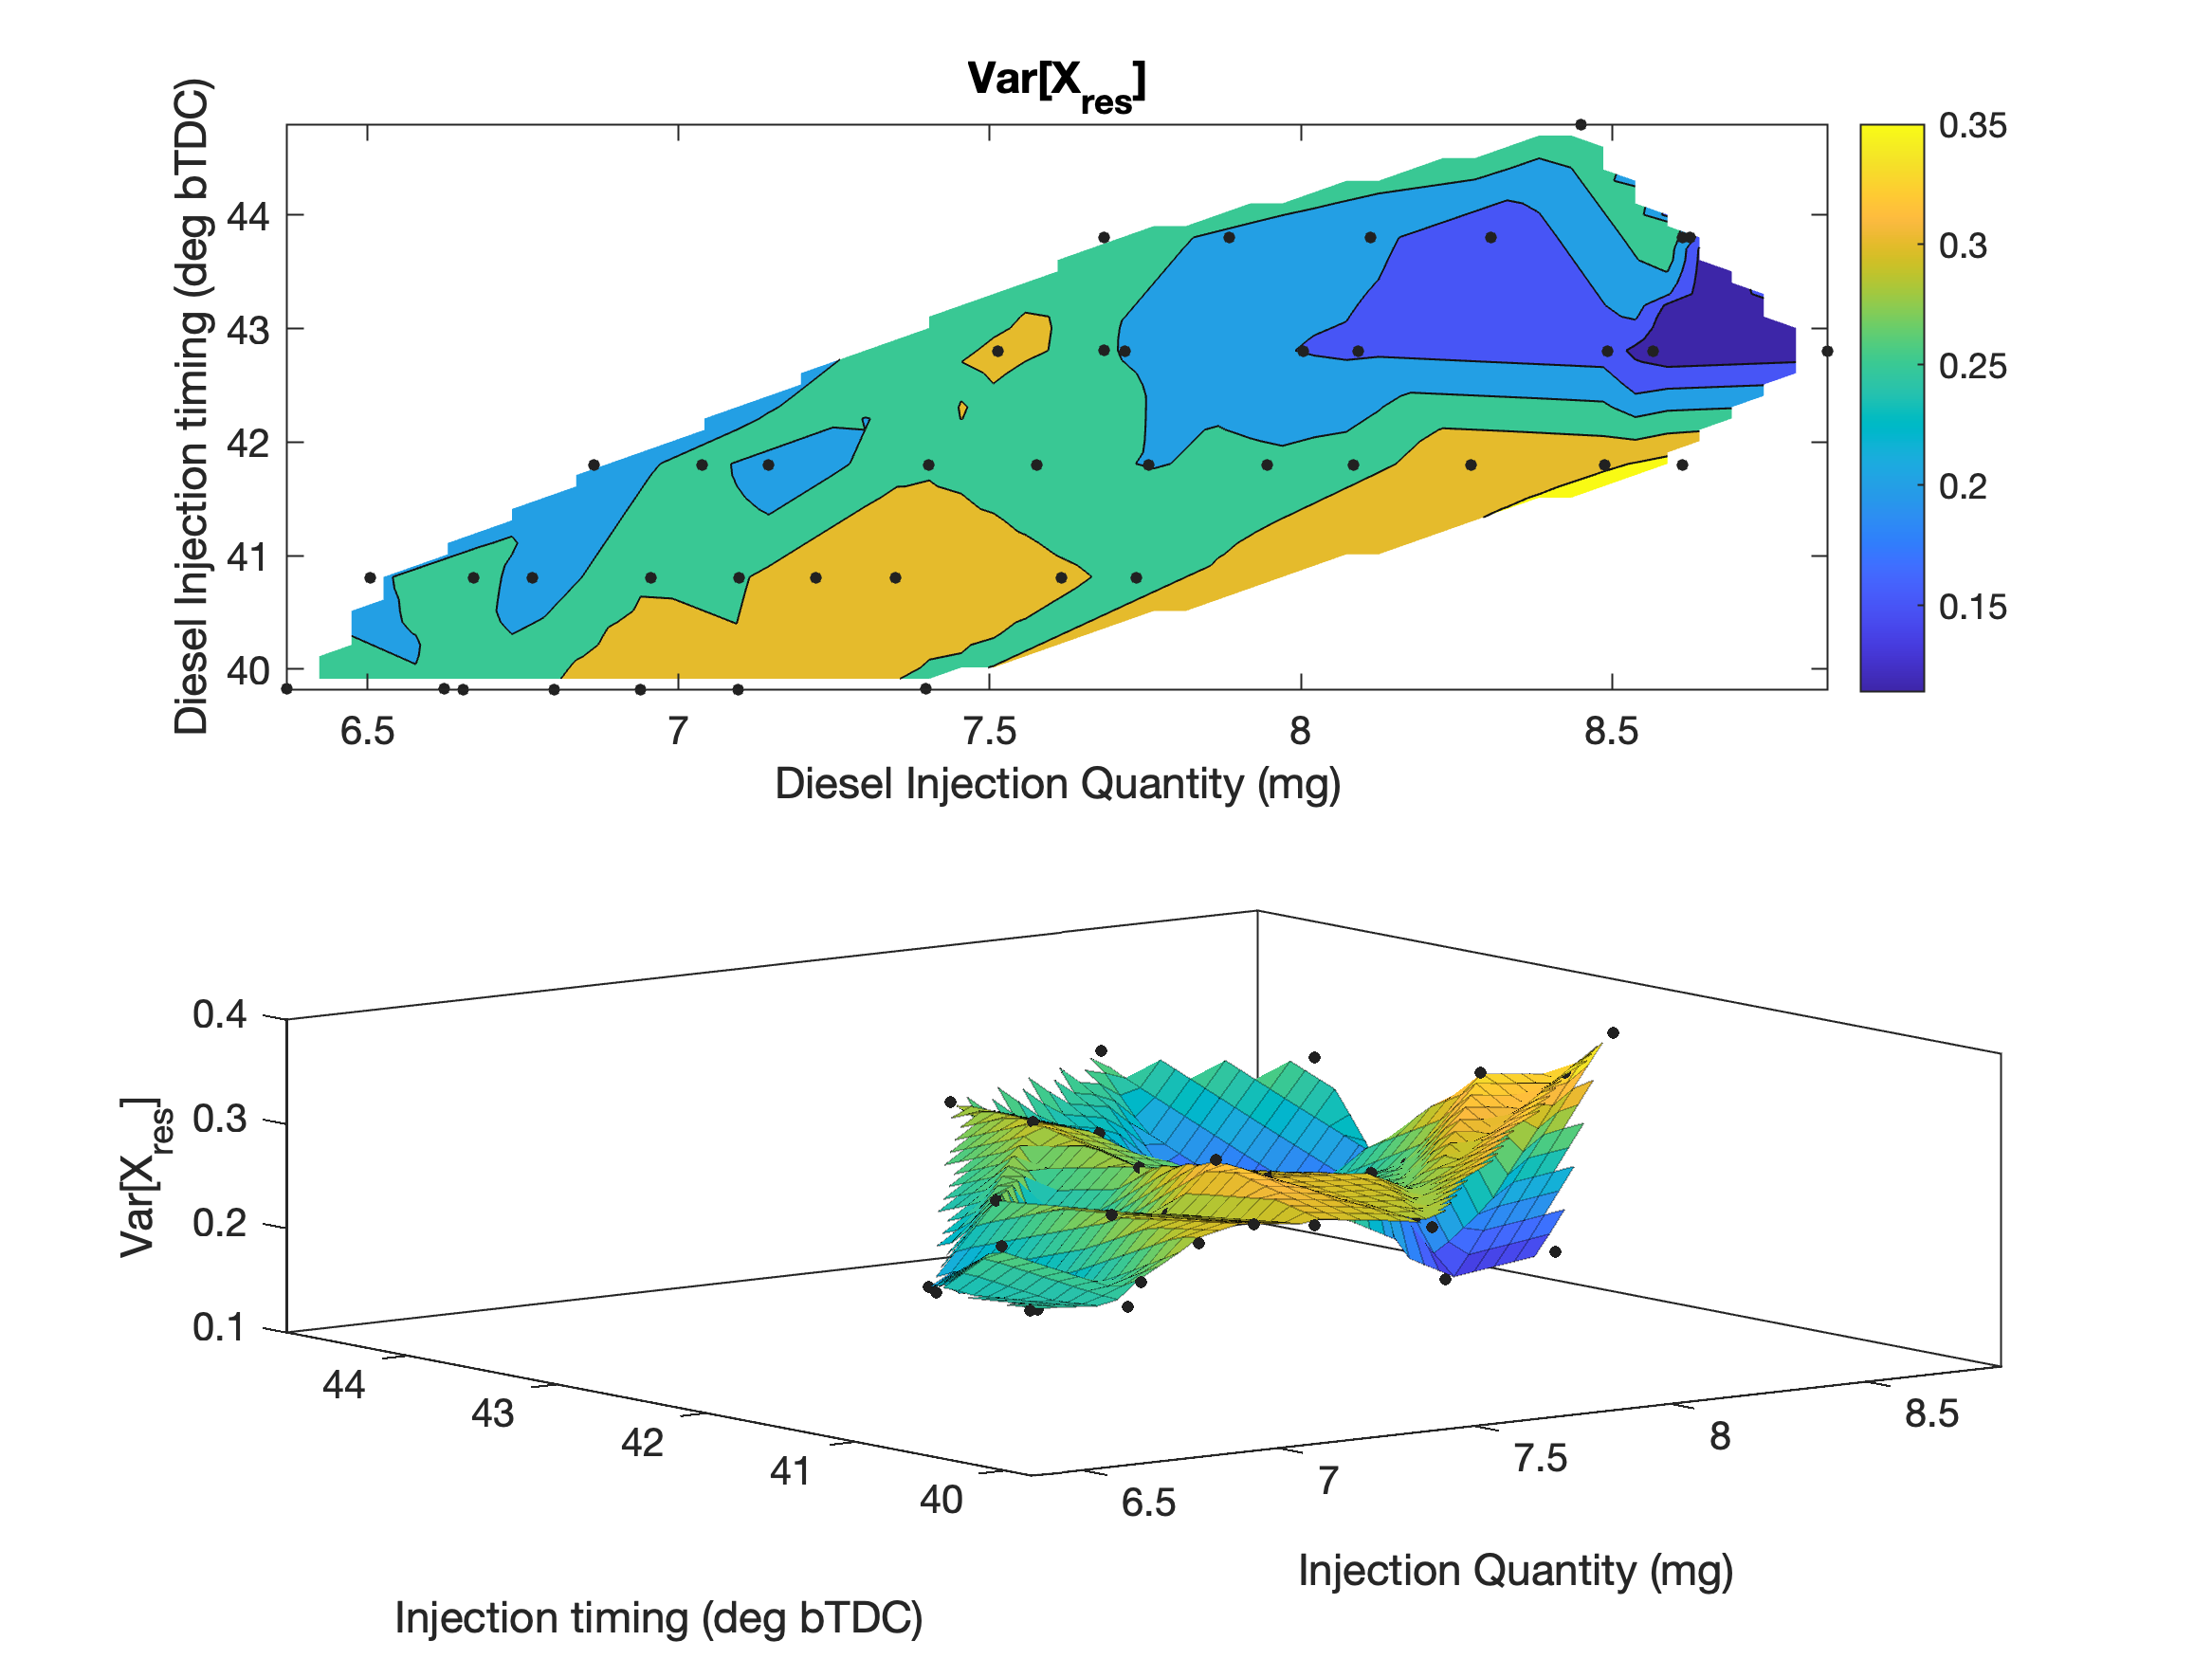
\includegraphics[width=0.36\textwidth]{../Model_Plots/Sigma_X_11.png}
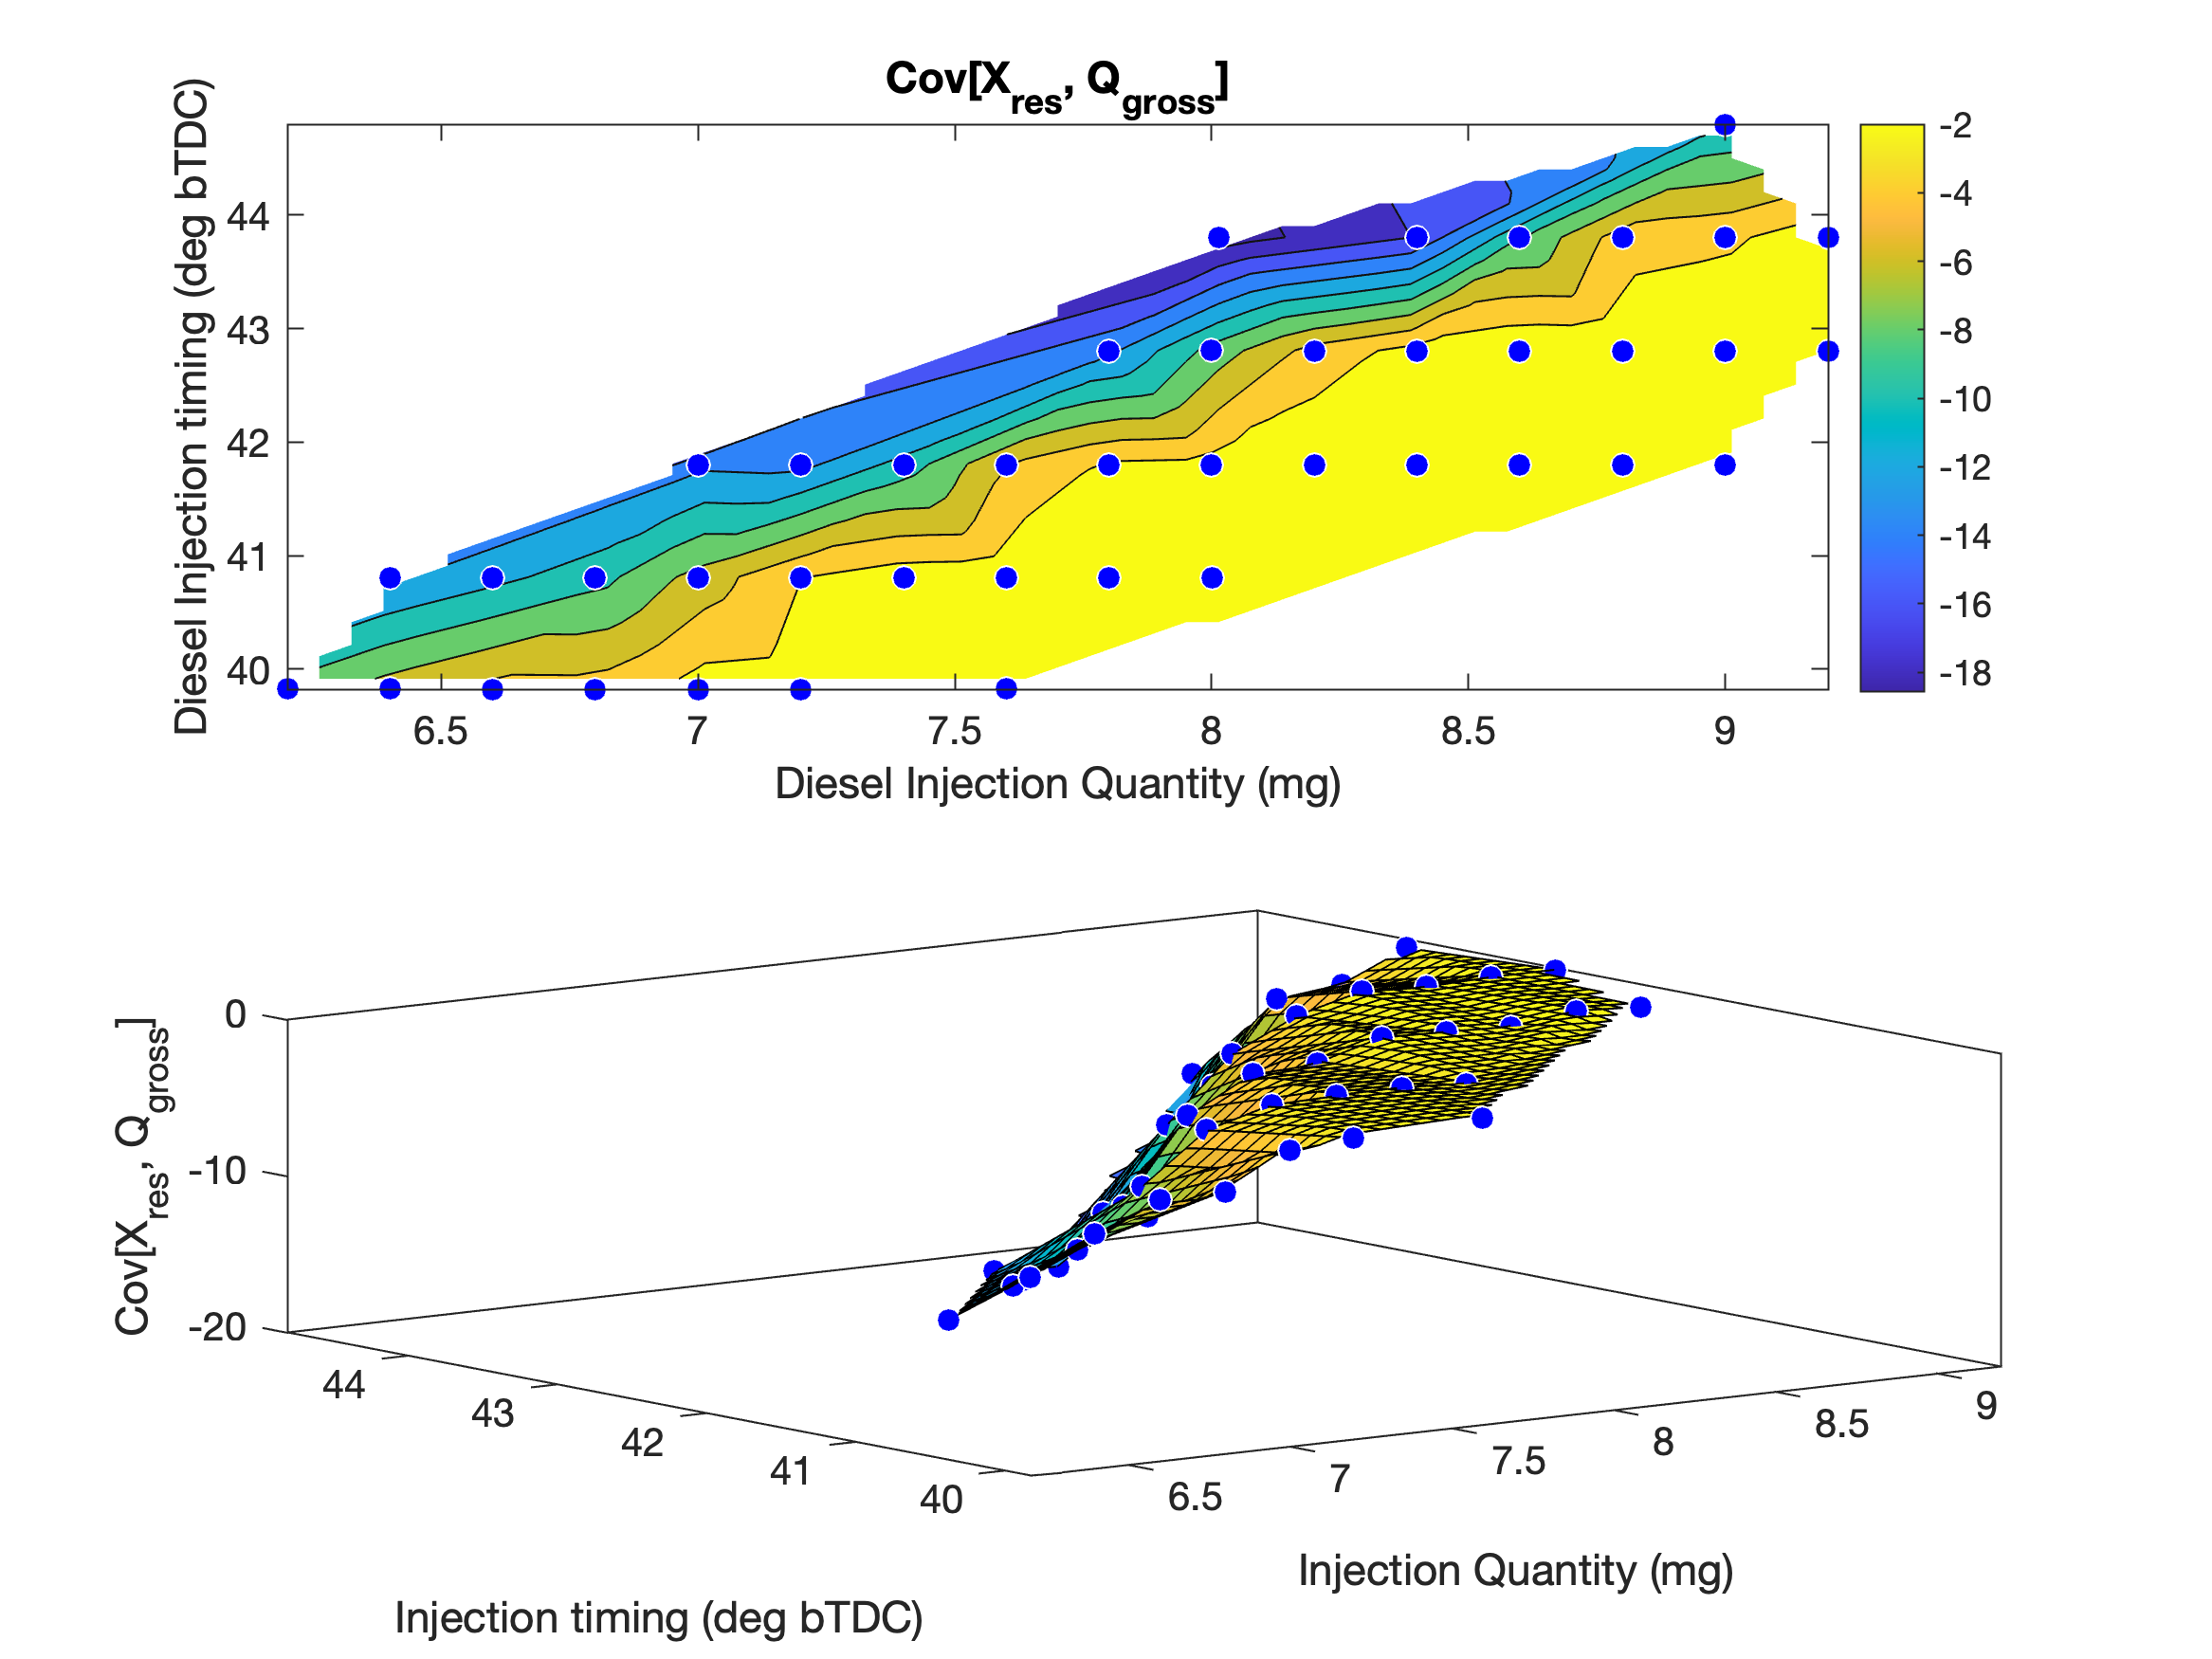
\includegraphics[width=0.36\textwidth]{../Model_Plots/Sigma_X_12.png}
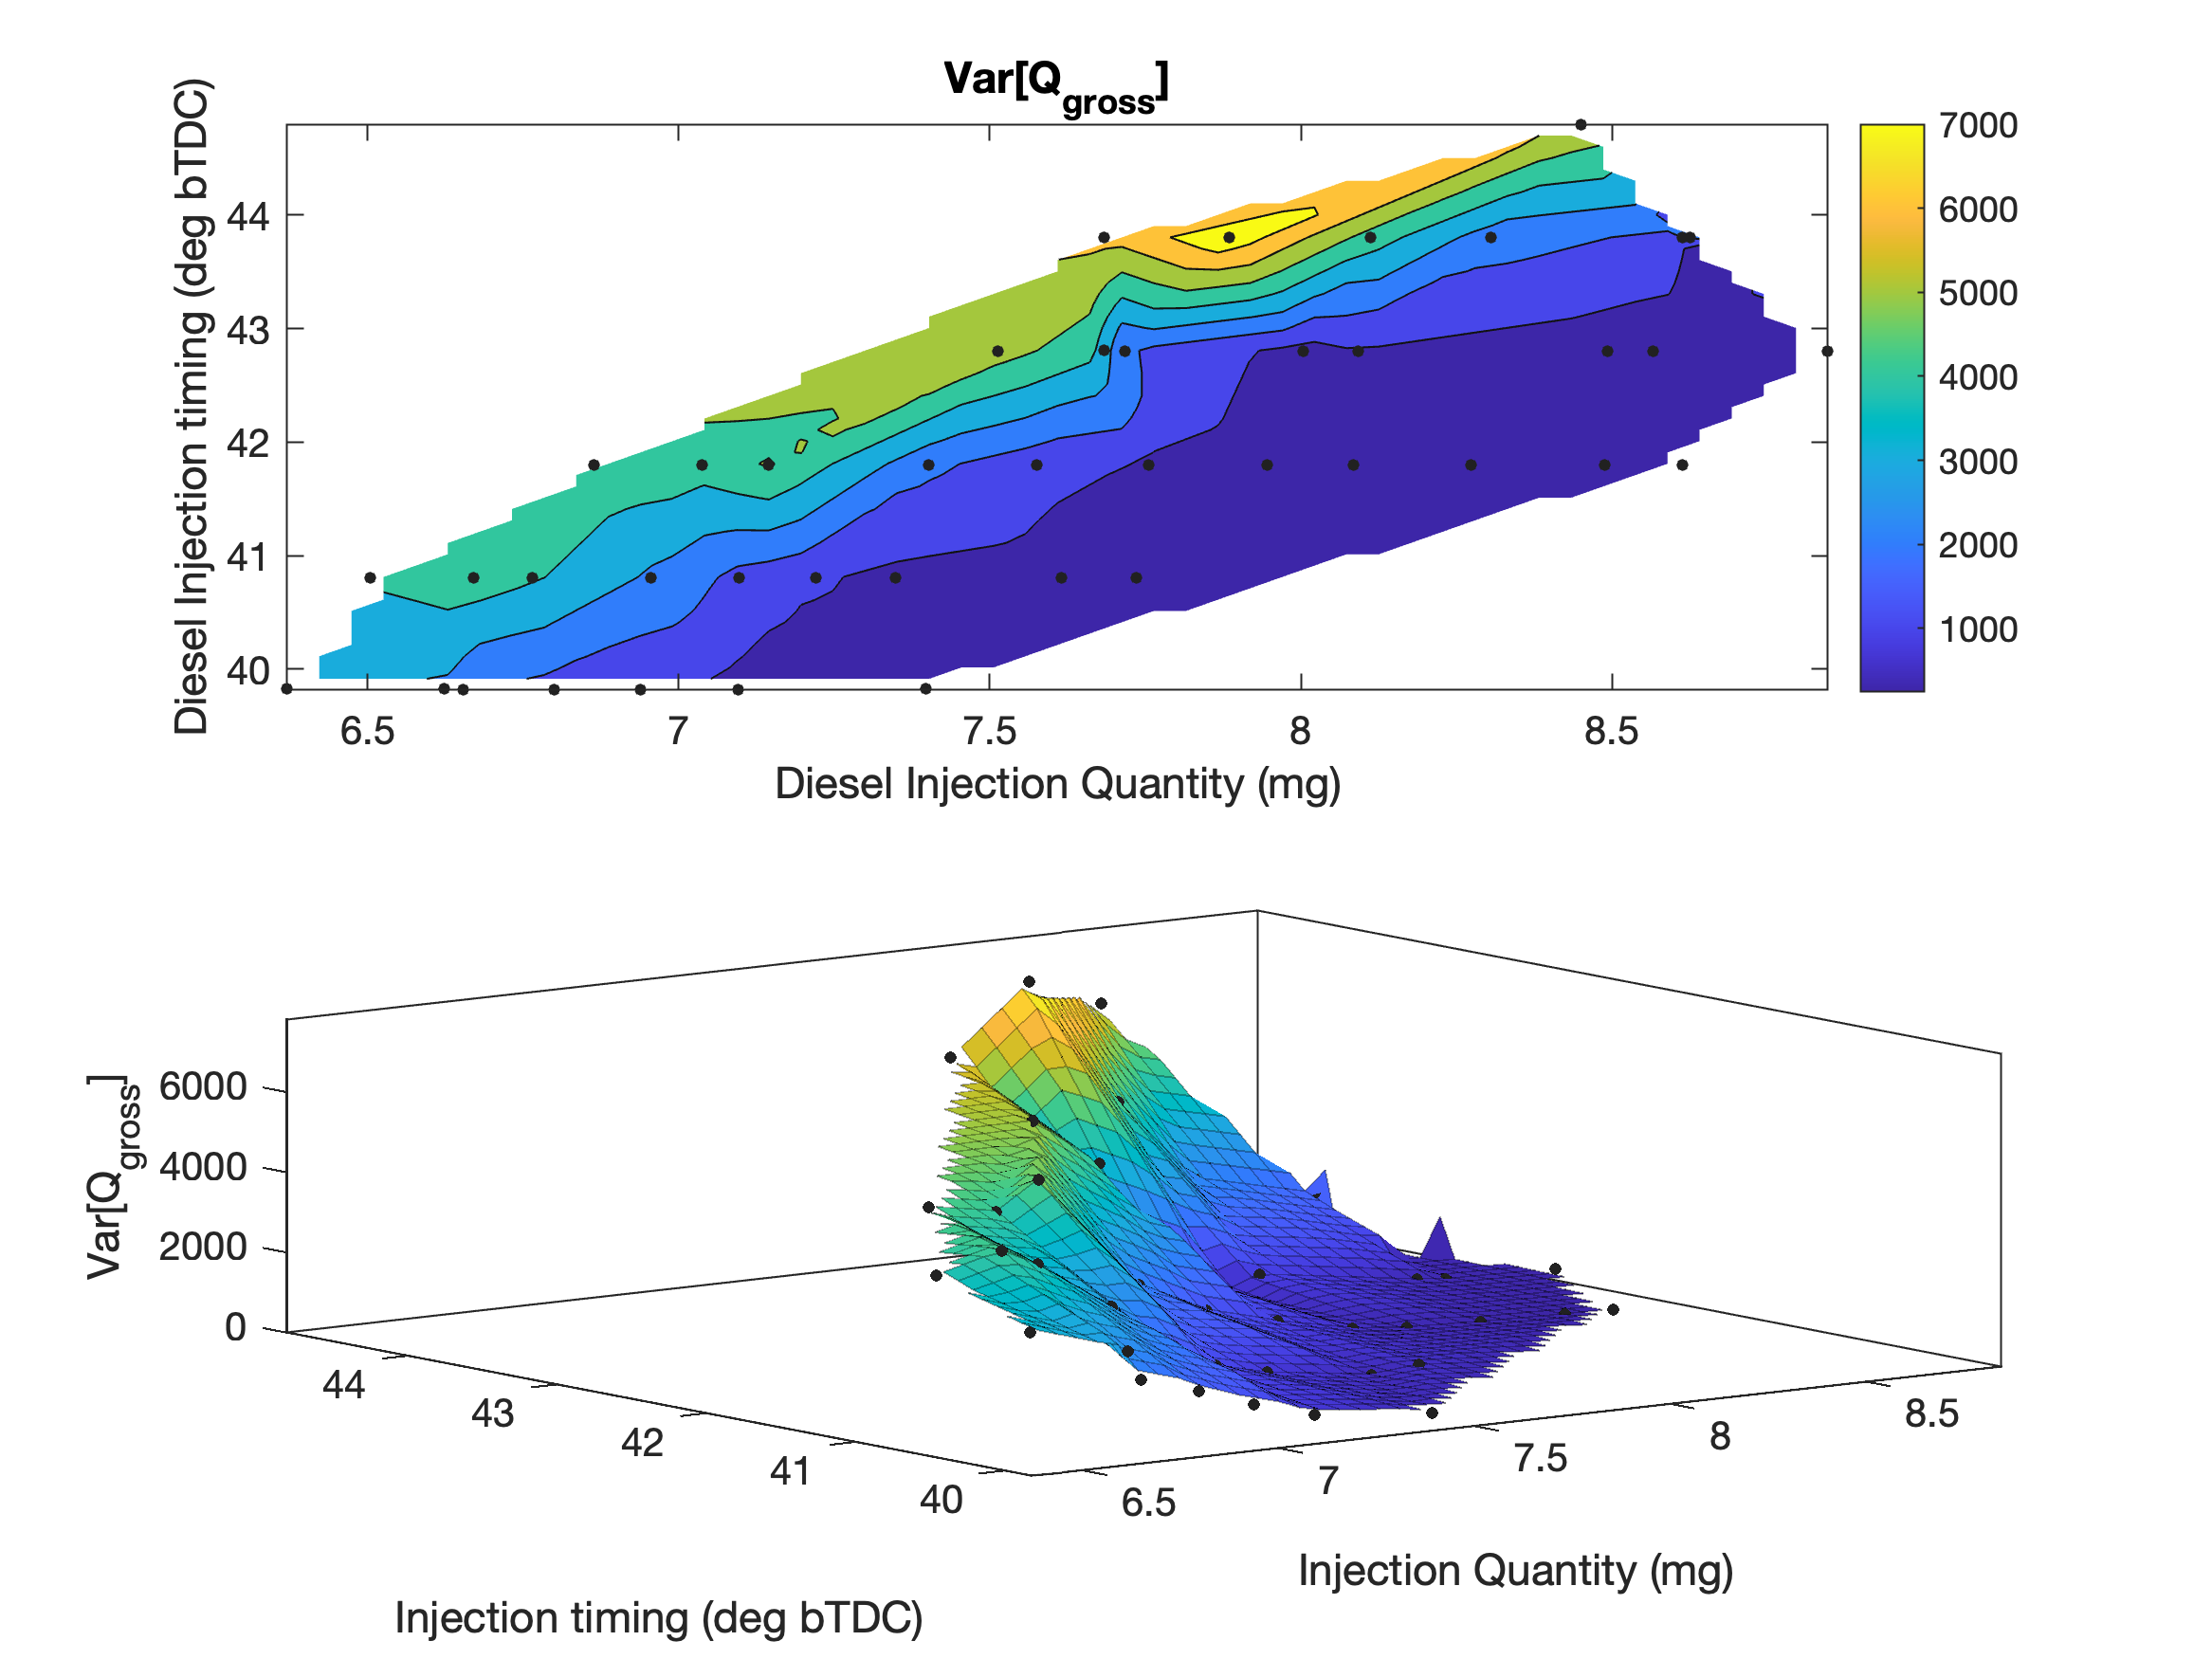
\includegraphics[width=0.36\textwidth]{../Model_Plots/Sigma_X_22.png}
\end{center}
\end{frame}

\begin{frame}
\frametitle{Model parameters $\mu_{CA50}$ and  $\Sigma_{CA50}$ as function of DI strategy}
\begin{center}
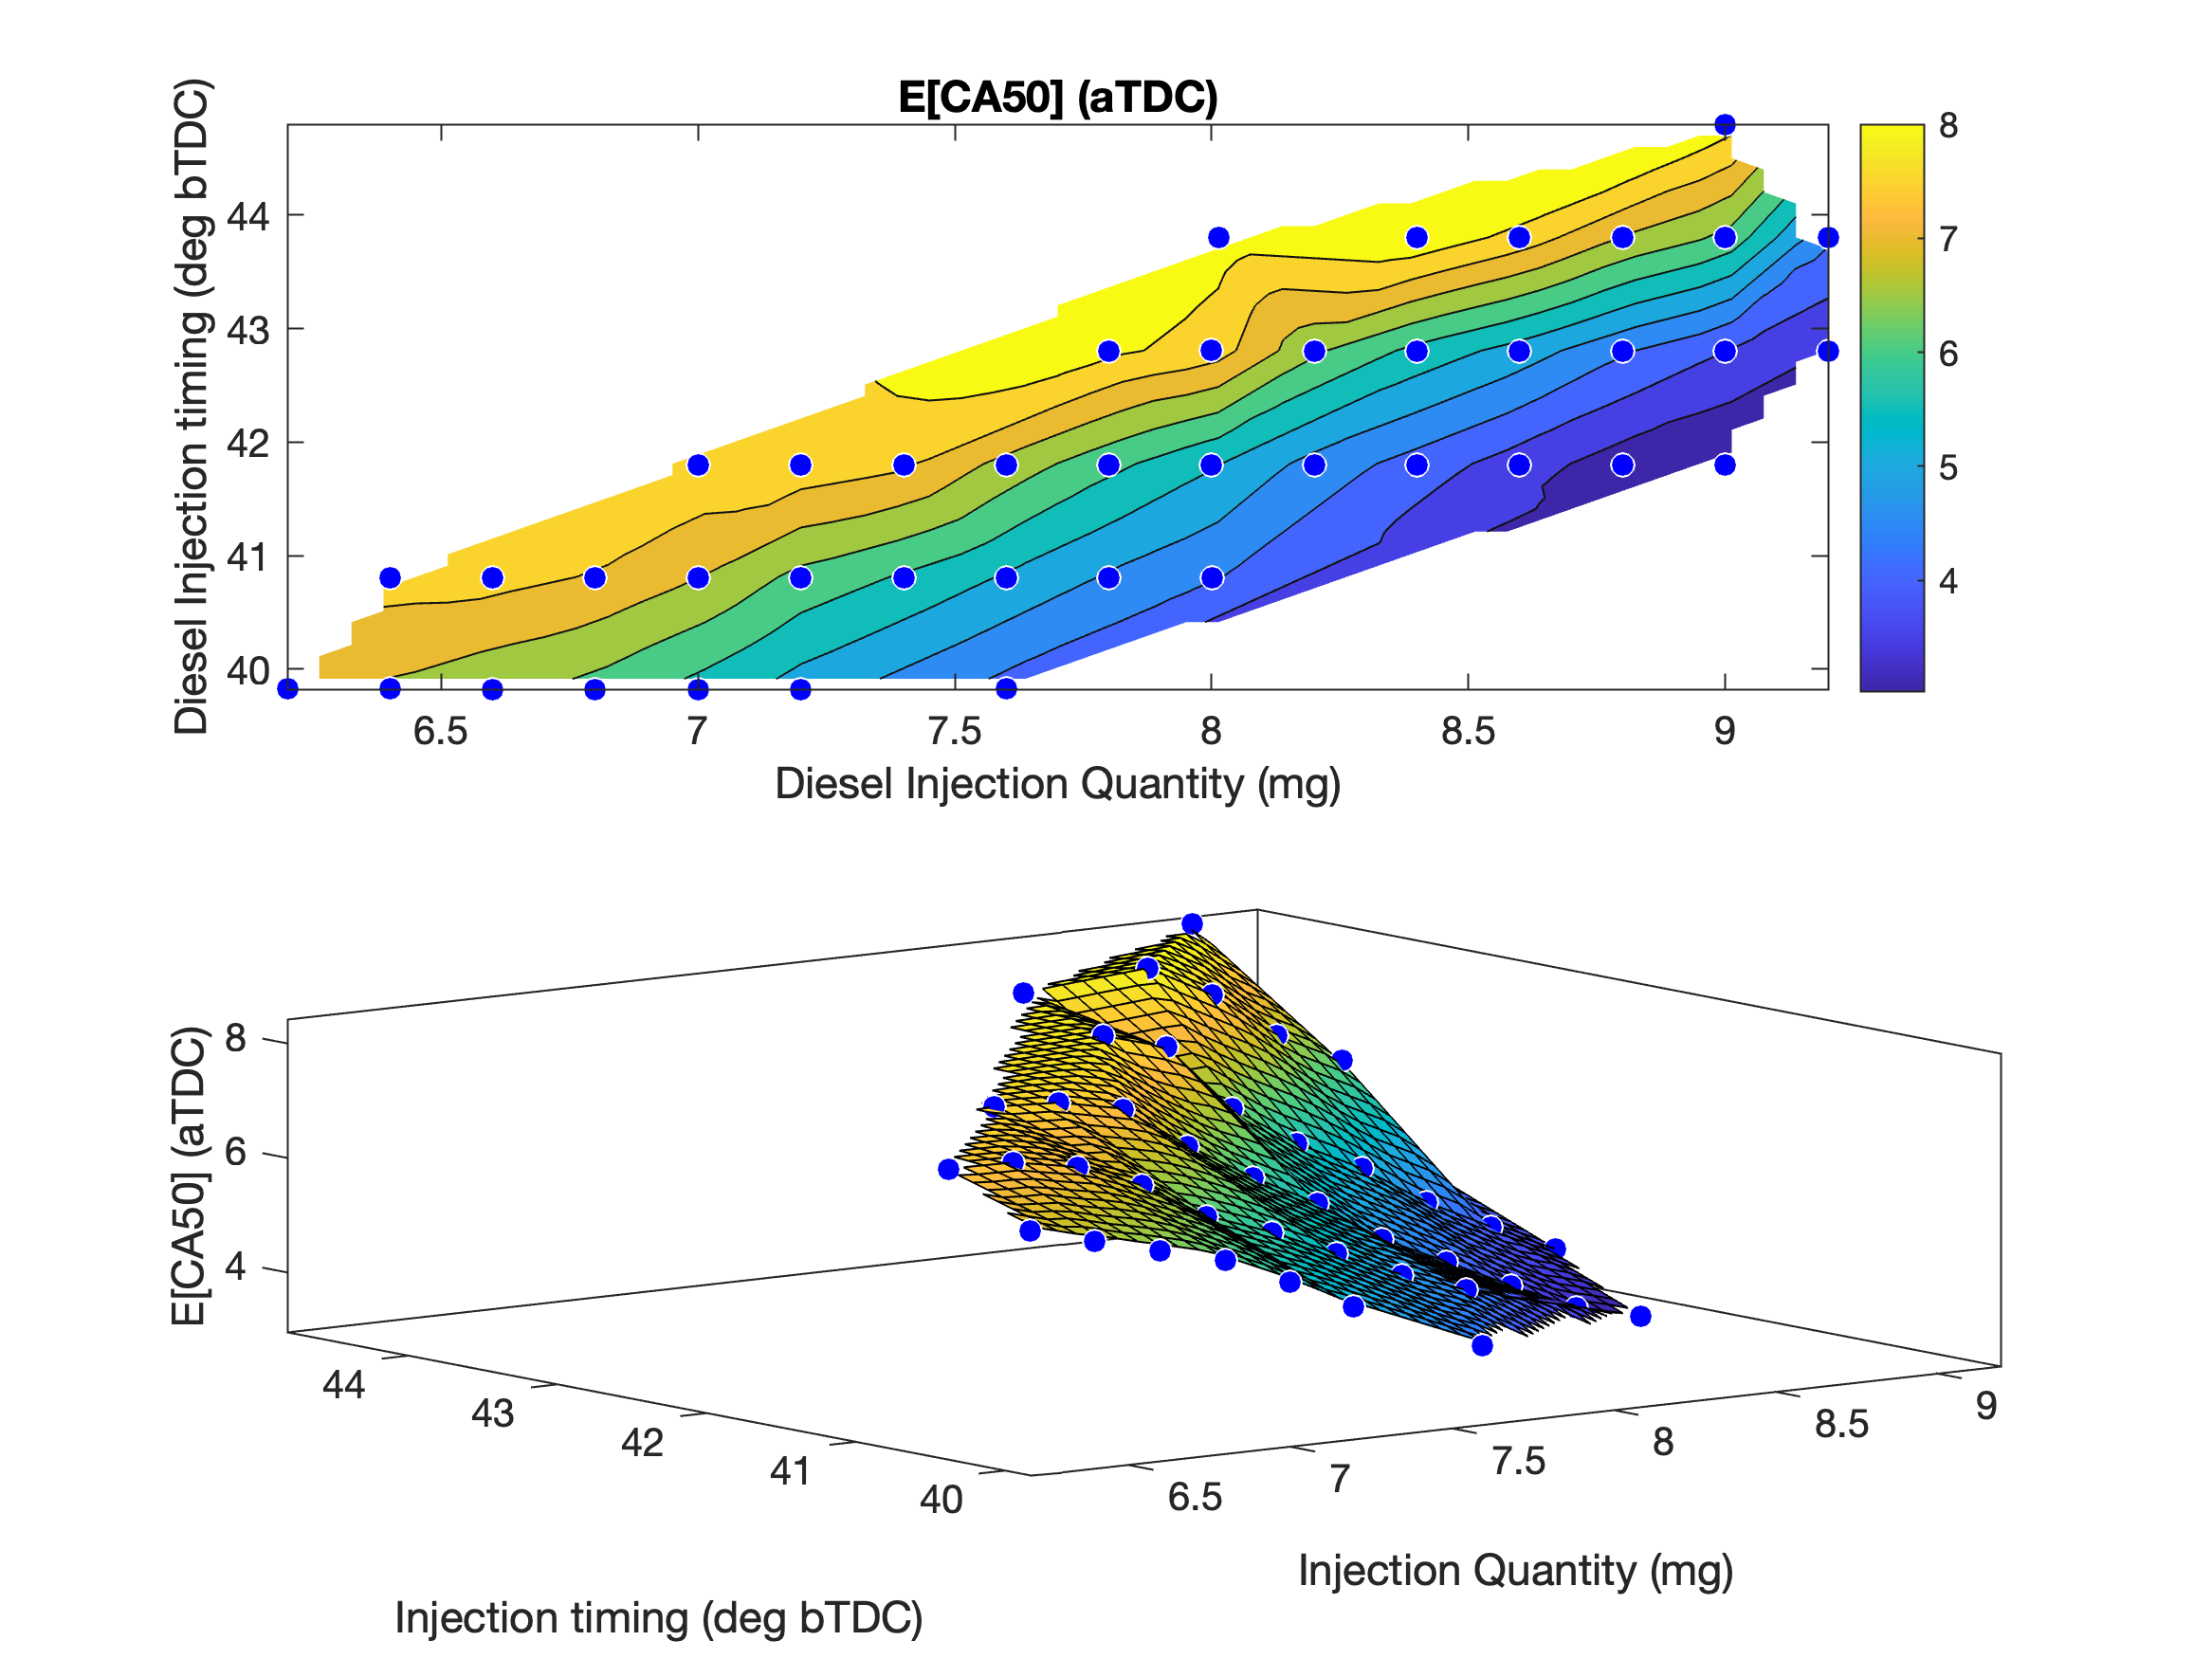
\includegraphics[width=0.49\textwidth]{../Model_Plots/mu_CA50.png}
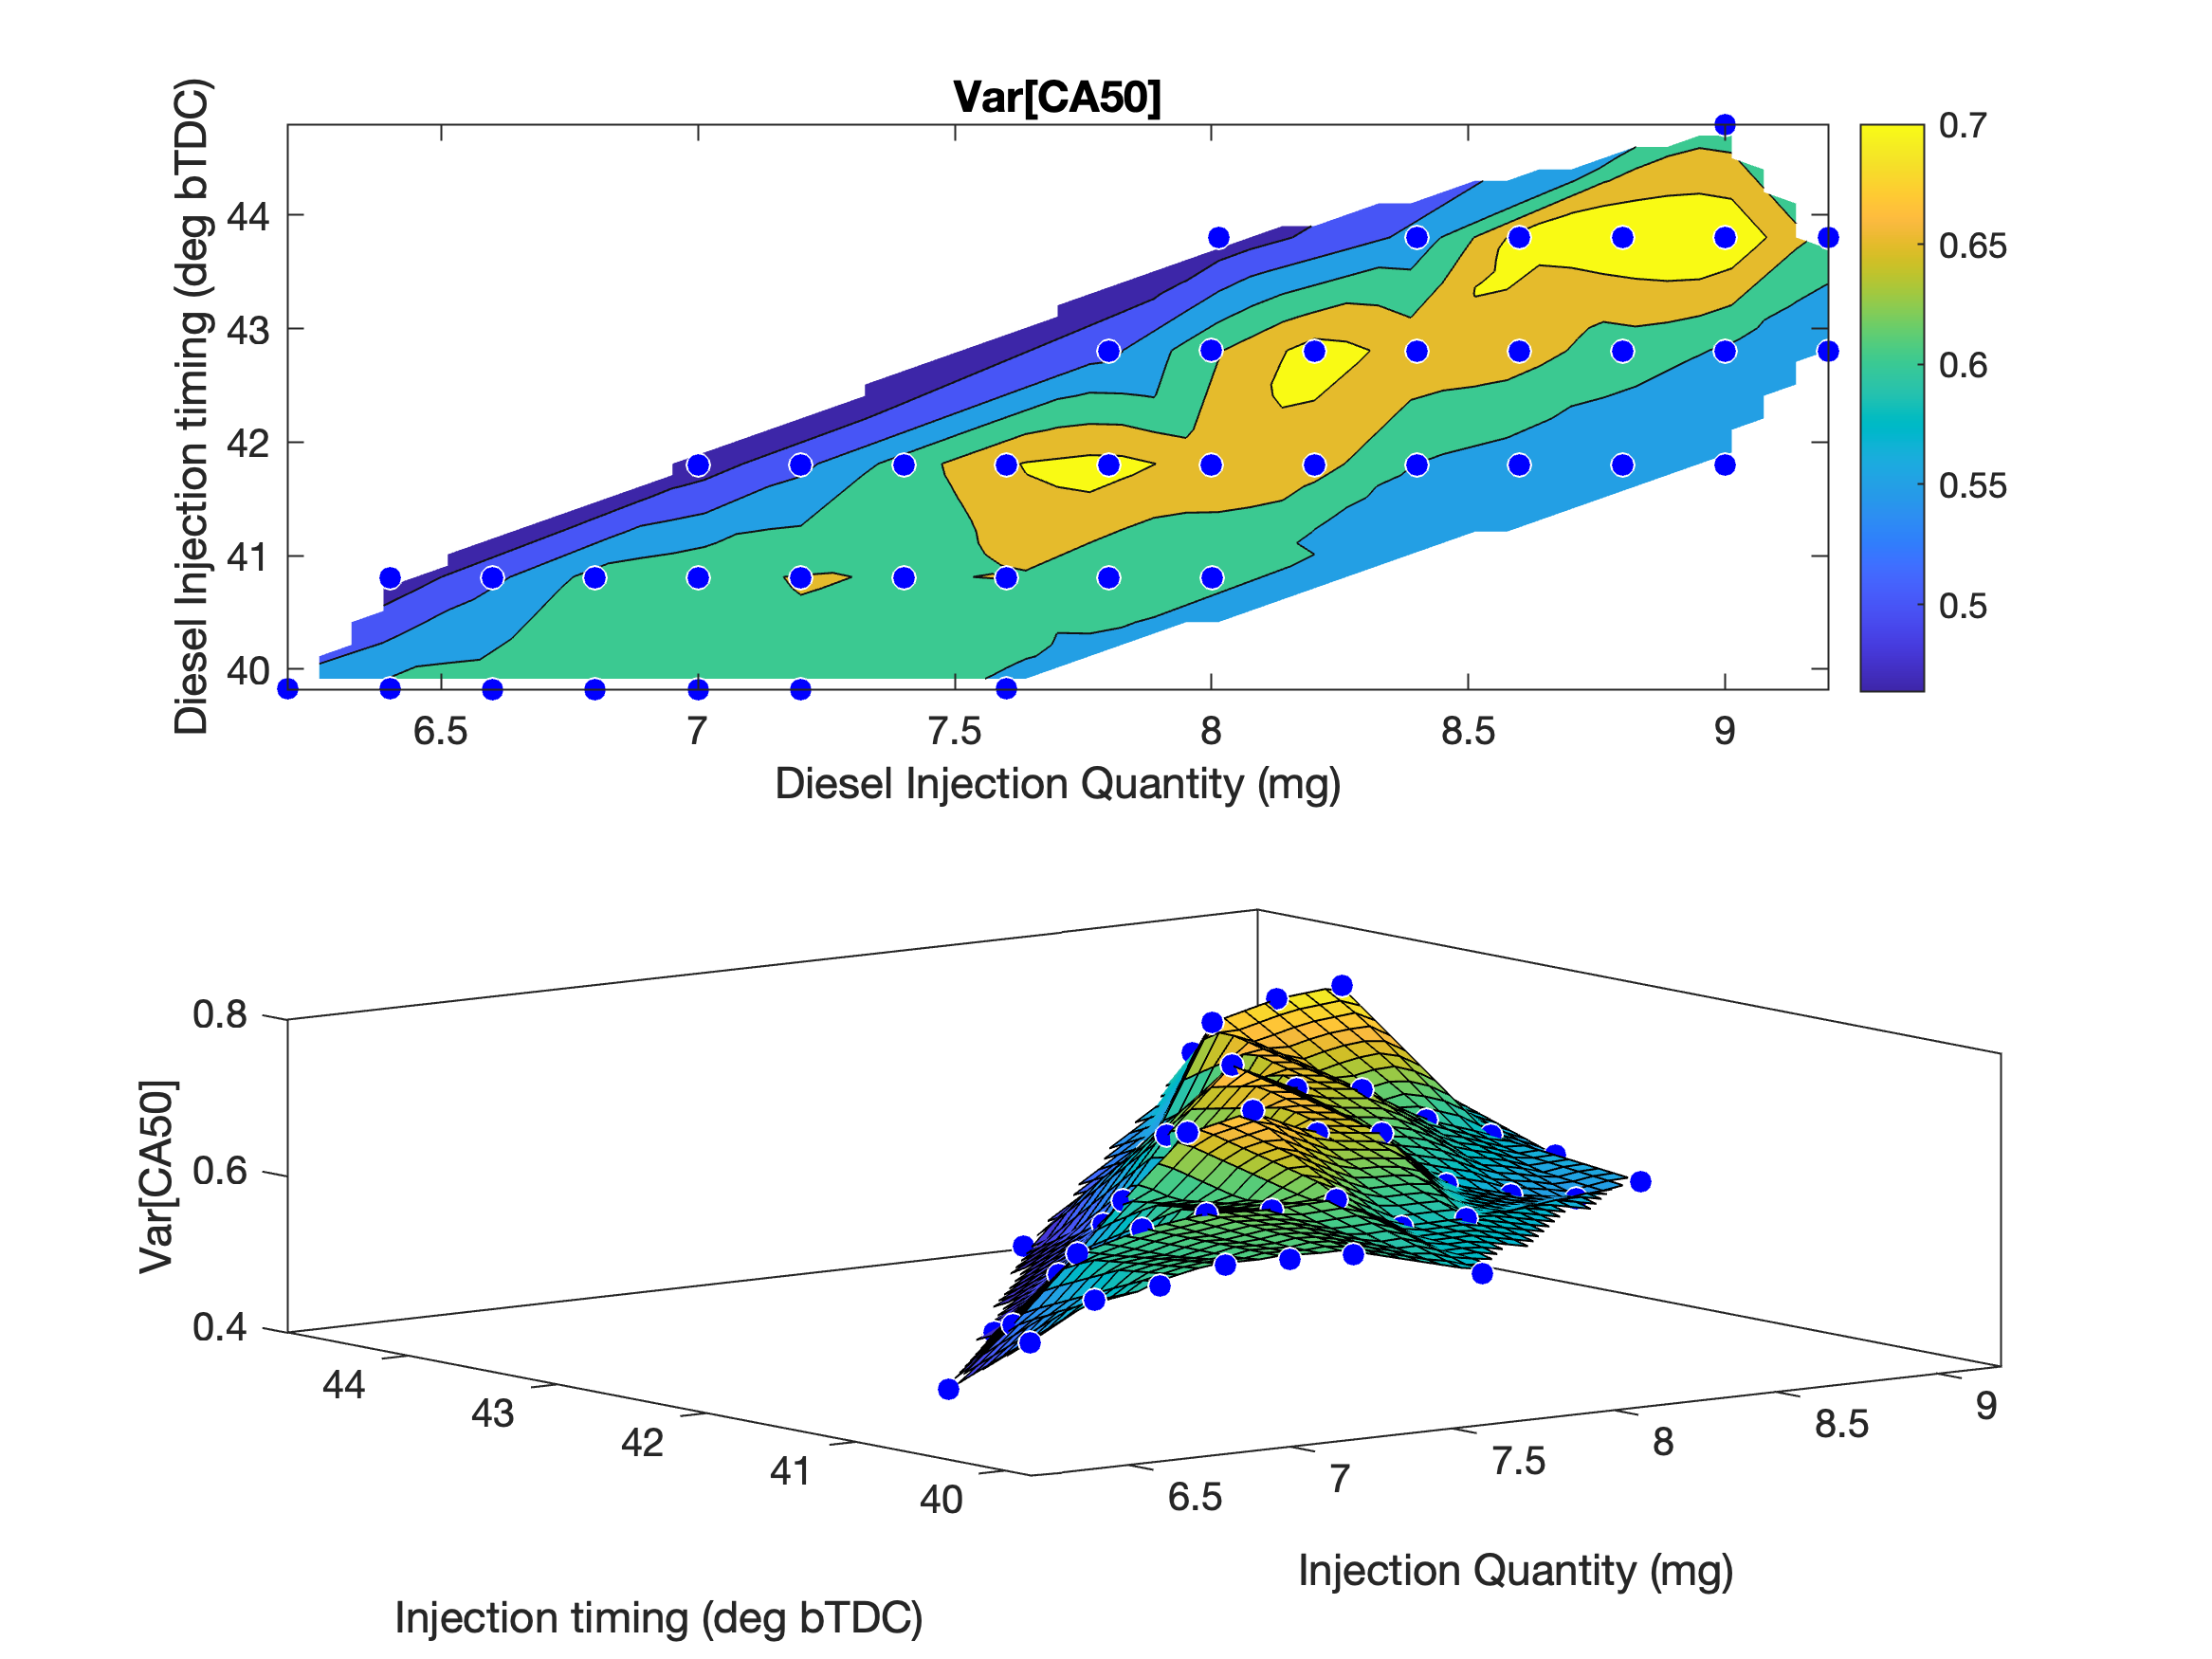
\includegraphics[width=0.49\textwidth]{../Model_Plots/Sigma_CA50.png}
\end{center}
\end{frame}

\begin{frame}
\frametitle{Model performance}
\begin{center}
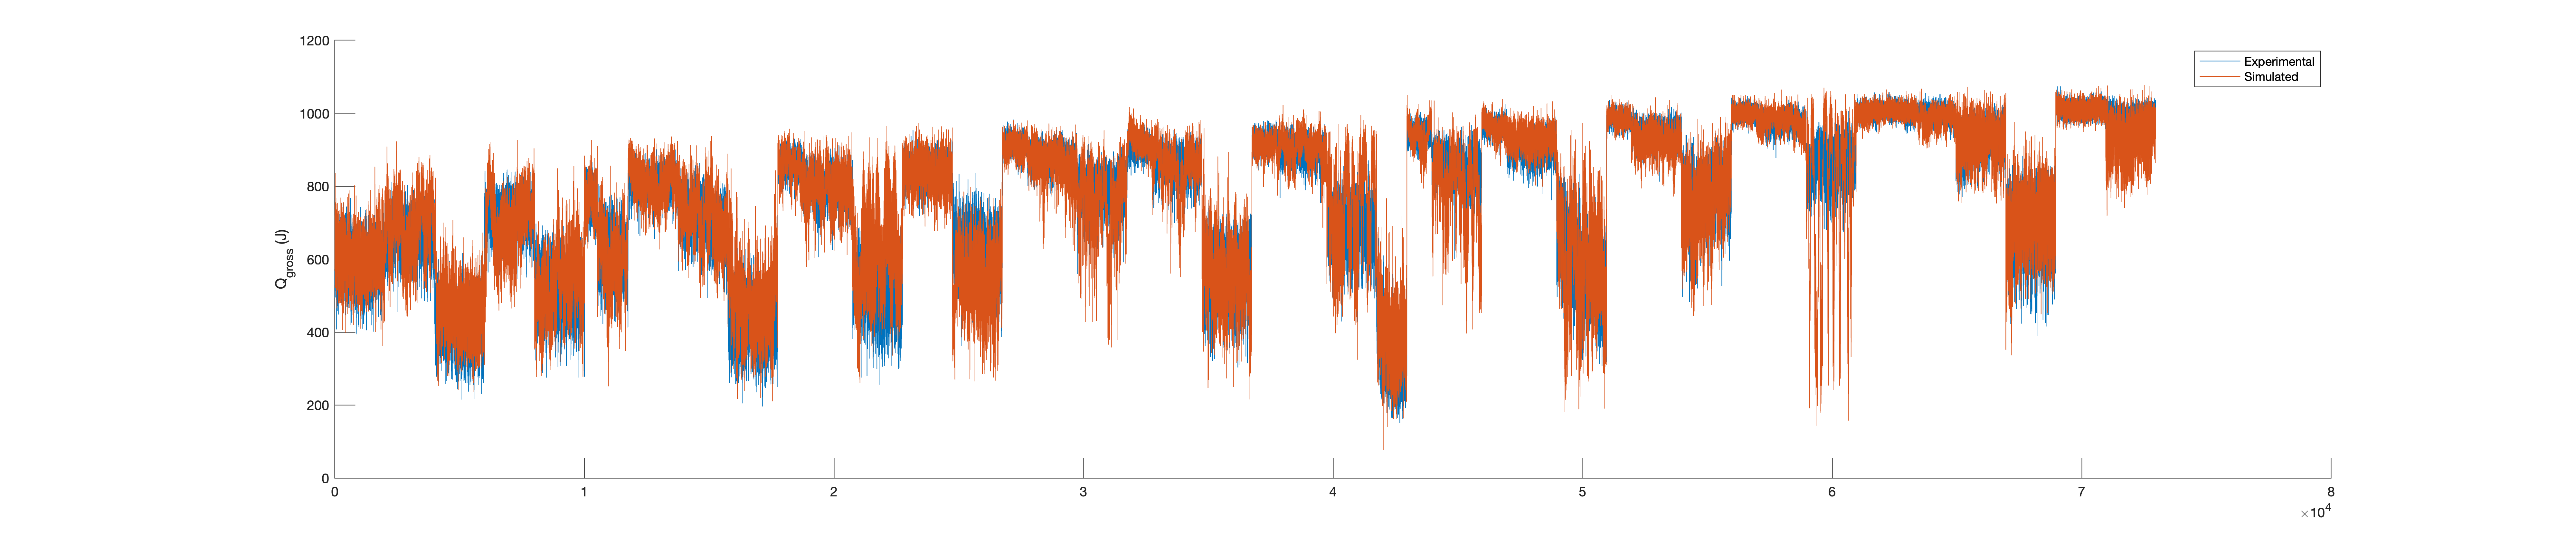
\includegraphics[trim=175 0 175 0, clip, width=\textwidth]{../Model_Plots/Q_gross_comparison.png}
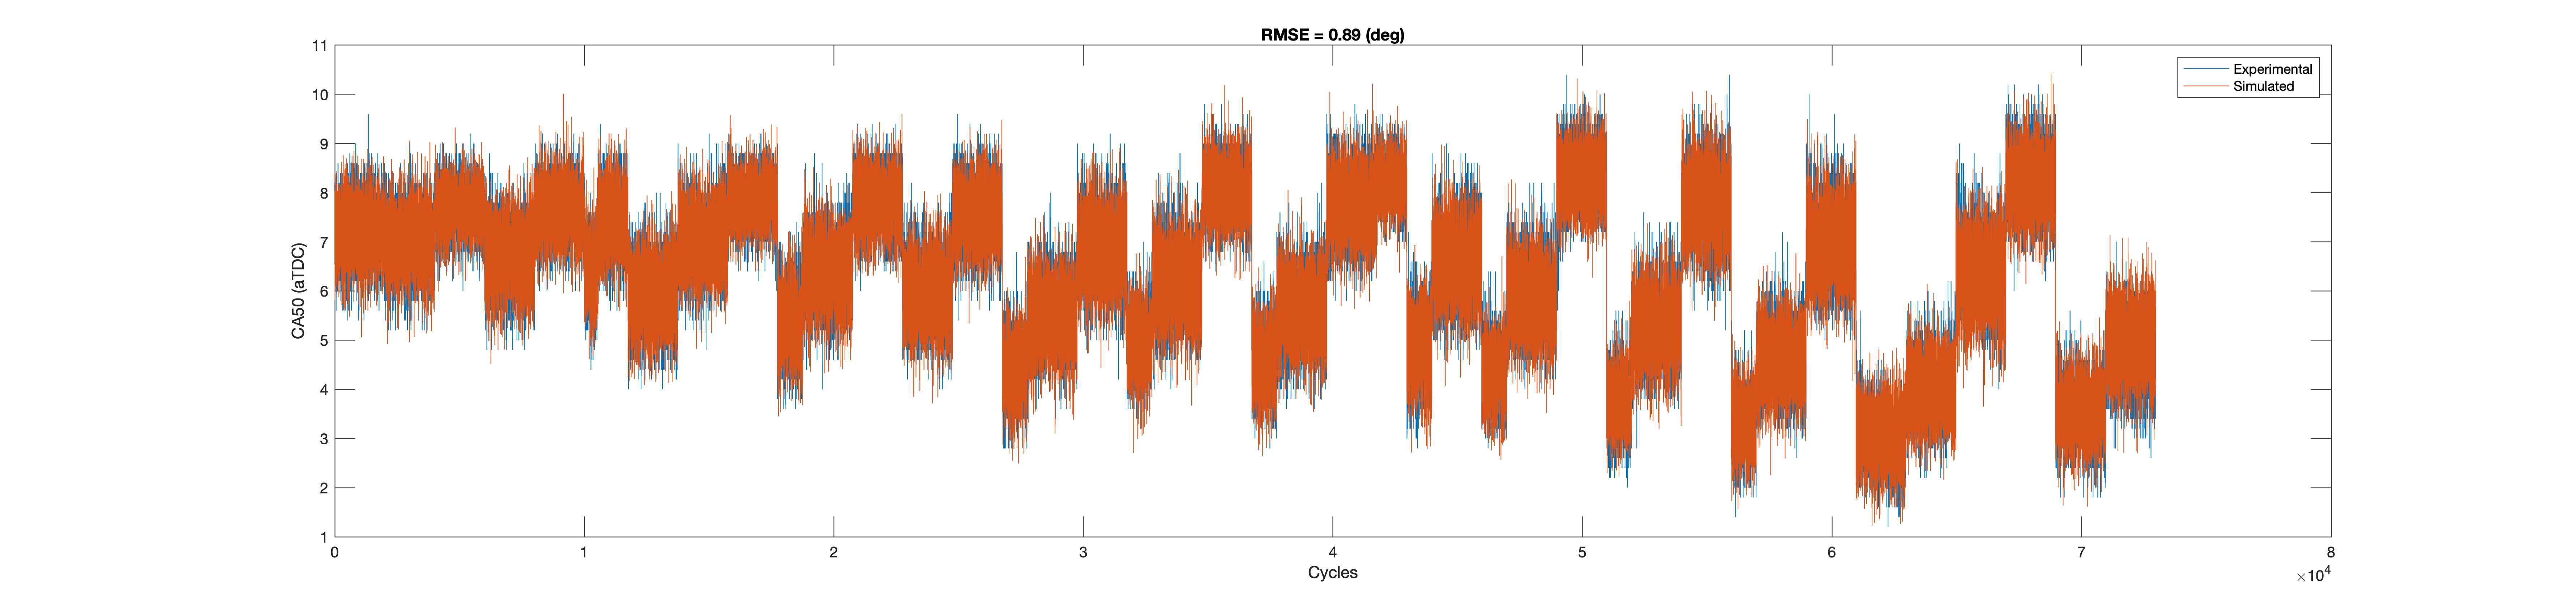
\includegraphics[trim=175 0 175 0, clip, width=\textwidth]{../Model_Plots/CA50_comparison.png}
\end{center}
\end{frame}

\end{document}